\documentclass[conference]{IEEEtran}
\IEEEoverridecommandlockouts
% The preceding line is only needed to identify funding in the first footnote. If that is unneeded, please comment it out.
\usepackage{cite}
\usepackage{amsmath,amssymb,amsfonts}
\usepackage{algorithmic}
\usepackage{graphicx}
\usepackage{textcomp}
\usepackage{xcolor}
\def\BibTeX{{\rm B\kern-.05em{\sc i\kern-.025em b}\kern-.08em
    T\kern-.1667em\lower.7ex\hbox{E}\kern-.125emX}}

\usepackage[bahasa]{babel}
\renewcommand{\IEEEkeywordsname}{Kata kunci}

\begin{document}

\title{Tugas VI (UTS)\\
{\footnotesize \textsuperscript{}}
\thanks{Identify applicable funding agency here. If none, delete this.}
}

\author{\IEEEauthorblockN{Johnny, Rian Sanjaya, Muhammad Riduan}
\IEEEauthorblockA{\textit{Faculty of Information Technology} \\
\textit{Institut Teknologi Batam}\\
Batam, Indonesia \\
Email: \{1822004, 1822012, 1822001\}@student.iteba.ac.id}
}

\maketitle

\begin{abstract}
Pada era transformasi digital, keamanan jaringan
menjadi semakin penting dan menarik untuk dikaji. Sistem
deteksi intrusi (IDS) merupakan bagian integral dari keamanan jaringan. Untuk meningkatkan keamanan jaringan, algoritma pembelajaran mesin dapat diterapkan untuk mendeteksi
dan mencegah serangan jaringan. Pemanfaatan kumpulan data
(dataset) seperti NSL-KDD, menjadi salah satu pendekatan untuk melatih model guna mendeteksi berbagai serangan jaringan.
Pada pekerjaan ini mahasiswa diharapkan dapat membandingkan performa dari beberapa algoritma yaitu Random Forest,
K-Neighbors, SVM dan Ensemble Learning
Algoritma Random Forest, K-Neighbors, SVM dan Ensemble
Learning dari masing-masing algoritma tersebut memiliki cara
klasifikasi yang berbeda, di sini kami akan membandingkan
kinerja masing-masing algoritma.
\end{abstract}

\begin{IEEEkeywords}
intrusion detection, Random Forest, K-Neighbors, SVM, Ensemble Learning, NSL-KDD dataset.
\end{IEEEkeywords}

\section{Pendahuluan}
pada era saat ini keamanan sistem maupun jaringan sangat
penting khusunya pengamanan informasi. Informasi pribadi
maupun informasi perusahaan sangat penting untuk dijaga
jika keamanan sistem atau jaringan rusak, maka harus segera
dilakukan perbaikan
Pengguna internet yang terus meningkat dari tahun ke
tahun tidak terlepas dari serangan yang timbul dari teknologi
jaringan seperti serangan malware infection. Oleh karena itu,
diperlukan keamanan dalam sistem komputer untuk mencegah
dari serangan.
IDS (Intrusion Detection System) merupakan sebuah aplikasi yang mampu mencatat kegiatan dalam suatu jaringan
dan menganalisa paket-paket yang dikirim melalui lalu lintas
jaringan secara realtime. Tujuan dari sistem ini yaitu mengawasi jika terjadi penetrasi ke dalam sistem, mengawasi traffic yang terjadi pada jaringan, mendeteksi anomaly terjadinya
penyimpangan dari sistem yang normal atau tingkah laku user.
Dalam melakukan deteksi serangan, dapat digunakan beberapa algoritma yaitu Random Forest, K-Neighbors, SVM dan
Ensemble Learning. Dan tujuan dari penelitian ini adalah untuk membandingkan performa dari masing-masing algoritma.

\section{Penjelasan Teori}

\subsection{Jaringan Komputer}

Jaringan komputer adalah jaringan telekomunikasi yang memungkinkan antar komputer untuk saling berkomunikasi dengan bertukar data. Tujuan dari jaringan komputer adalah agar dapat mencapai tujuannya, setiap bagian dari jaringan komputer dapat meminta dan memberikan layanan.

\begin{figure}
\centering

\includegraphics[width=.4\textwidth]{Gambar/gambar7.jpg}
\caption{Contoh keamanan komputer}
\end{figure}

\subsection{Random Forest}\label{AA}
Random forest adalah suatu algoritma yang digunakan pada klasifikasi data dalam jumlah yang besar. Klasifikasi random forest dilakukan melalui penggabungan pohon dengan melakukan training pada sampel data yang dimiliki.
Keuntungan Random Forest adalah sebagai berikut [1]:

1) Hutan yang dihasilkan dapat disimpan untuk referensi
di masa mendatang.

2) Hutan acak mengatasi masalah penyesuaian.

3) Dalam akurasi RF dan kepentingan variabel secara
otomatis dihasilkan.

Flowchart dari proses pemodelan algoritma Random Forest
dapat dilihat pada “Gambar. 1”.

\begin{figure}
\centering
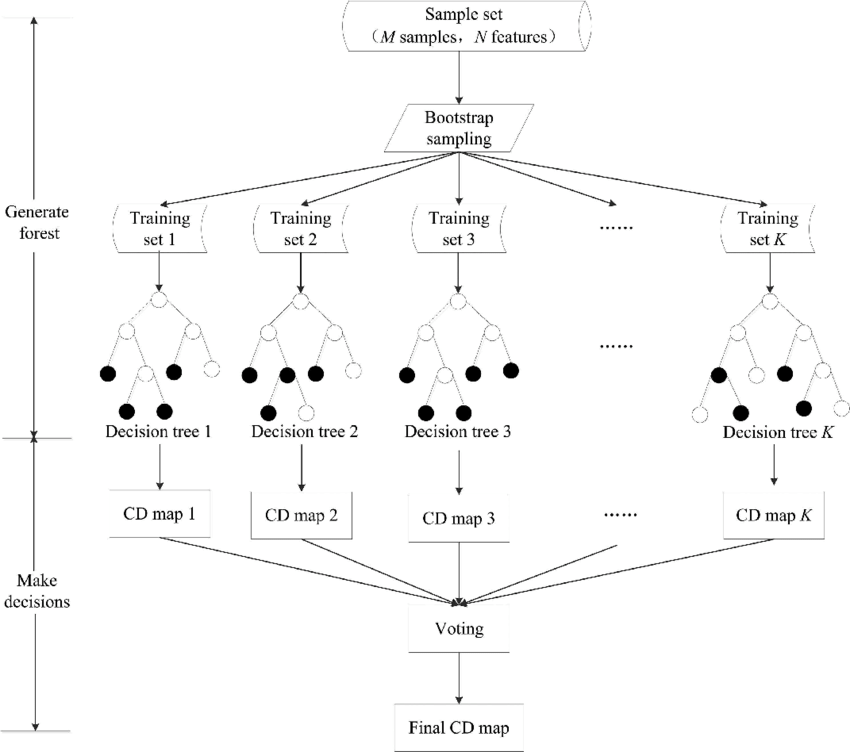
\includegraphics[width=.4\textwidth]{Gambar/gambar1.png}
\caption{Flowchart Algoritma Random Forest}
\end{figure}

\subsection{K-Nearest Neighbors}

Algoritme k tetangga terdekat adalah sebuah metode untuk melakukan klasifikasi terhadap objek berdasarkan data pemelajaran yang jaraknya paling dekat dengan objek tersebut. Data pemelajaran digambarkan ke ruang berdimensi banyak dengan tiap-tiap dimensi mewakili tiap ciri/fitur dari data.

\noindent\emph{Euclidean Distance}\\
Untuk mendefinisikan jarak antara dua titik yaitu titik pada data training (x) dan titik pada data testing (y), maka digunakan rumus \emph{Euclidean}\cite{nurhadi2017aplikasi}, yaitu:

% ini memasukkan rumus
\begin{equation*}
d(x,y)=\sqrt{\sum^{n}_{i=1} (x_i-y_i)^2}
\label{eq1}
\end{equation*}
% sampai sisi

dimana:

$d$ = jarak antara 2 titik

$x$ = data uji

$y$ = data latih

$i$ = merepresentasikan nilai atribut

$n$ = merupakan dimensi atribut.\vspace{10pt}

\noindent\emph{City Block Distance}\\
\emph{City Block Distance} umumnya dihitung antara 2 koordinat objek yang berpasangan. Ini adalah penjumlahan dari perbedaan absolut antara 2 koordinat. \emph{City Block Distance} 2-titik a dan b dengan dimensi k dihitung secara matematis menggunakan rumus berikut ini:

\begin{equation*}
d_{ij}=\sum^{k}_{i=1} | a_i-b_i |
\label{eq2}
\end{equation*}

\noindent\emph{Manhattan Distance}\\
\emph{Manhattan Distance} merupakan salah satu pengukuran yang paling banyak digunakan meliputi penggantian perbedaan kuadrat dengan menjumlahkan perbedaan \emph{absolute} dari variabel-variabel. Fungsi ini hanya akan menjumlahkan selisih nilai x dan y dari dua buah titik.
\vspace{10pt}

\noindent\emph{Minkwoski Distance}\\
\emph{Minkwoski Distance} adalah metrik dalam ruang vektor bernorma yang dapat dianggap sebagai generalisasi dari kedua jarak \emph{Euclidean} dan jarak \emph{Manhattan}. Jarak \emph{Minkowski} antara dua variabel X dan Y didefinisikan sebagai:

\begin{equation*}
d = (\sum^{n}_{i=1} | X_i-Y_i |^p)^{1/p}
\label{eq3}
\end{equation*}

Kasus di mana $p$ = 1 setara dengan jarak \emph{Manhattan} dan kasus di mana $p$ = 2 setara dengan jarak \emph{Euclidean}.
Flowchart dari proses pemodelan algoritma \emph{K-nearest neighbors} dapat dilihat pada ``Gambar. 2''.\vspace{6pt}
\begin{figure}
\centering
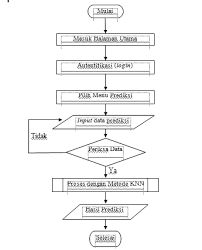
\includegraphics[width=.4\textwidth]{Gambar/gambar3.png}
\caption{Flowchart Algoritma K-Nearest Neighbors}
\end{figure}


\subsection{Algoritma SVM}
Support Vector Machine (SVM) adalah algoritme supervised yang berupa klasifikasi dengan cara membagi data menjadi dua kelas menggunakan garis vektor yang disebut hyperplane (Octaviani, et al., 2014). Pada permasalahan yang kompleks atau permasalahan dengan parameter yang banyak, metode ini sangat baik untuk digunakan.

Teori SVM berasal dari statistik dan prinsip dasar SVM adalah menemukan \emph{hyperplane} linier yang optimal dalam ruang fitur yang secara maksimal memisahkan dua kelas target.

Dalam kaitannya dengan fungsi kernel, fungsi diskriminan mengambil bentuk berikut:

\begin{equation*}
f(x) = \sum^{n}_i \alpha_ik(x,x_i)+b
\label{eq4}
\end{equation*}

Dalam pekerjaan ini, kernel \emph{Gaussian} telah digunakan
untuk membangun pengklasifikasi SVM.\\ \emph{Gaussian} kernel:

\begin{equation*}
K(x_i,x_j) = exp\left (- \frac{||x_i-x_j||^2}{2\sigma} \right )
\label{eq5}
\end{equation*}

\noindent dimana $\sigma$ adalah lebar fungsi.

Fungsi kernel dan parameternya harus dipilih untuk membangun pengklasifikasi SVM. Melatih SVM menemukan \emph{hyperplane} margin besar, yaitu menetapkan parameter $\alpha$.

Flowchart dari proses pemodelan algoritma SVM dapat dilihat pada ``Gambar. 3''.\vspace{6pt}

\begin{figure}
\centering
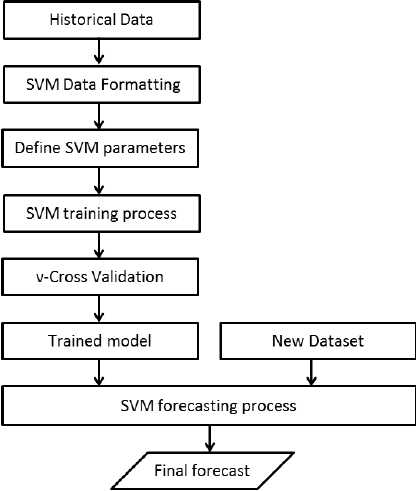
\includegraphics[width=.4\textwidth]{Gambar/gambar2.png}
\caption{Flowchart Algoritma SVM}
\end{figure}

\subsection{Ensemble Learning}

Metode ensemble atau metode ansamble adalah algoritma dalam pembelajaran mesin (machine learning) dimana algoritma ini sebagai pencarian solusi prediksi terbaik dibandingkan dengan algoritma yang lain karena metode ensemble ini menggunakan beberapa algoritma pembelajaran untuk pencapaian solusi prediksi yang lebih baik daripada algoritma yang bisa diperoleh dari salah satu pembelajaran algoritma kosituen saja. Tidak seperti ansamble statistika didalam mekanika statistika biasanya selalu tak terbatas. Ansemble Pembelajaran hanya terdiri dari seperangkat model alternatif yang bersifat terbatas, namun biasanya memungkinkan untuk menjadi lebih banyak lagi struktur fleksibel yang ada diantara alternatif model itu sendiri.

Metode ini adalah menggabungkan beberapa fitur dengan pembelajaran \emph{Ensemble}.

Flowchart dari proses pemodelan algoritma \emph{Ensemble Learning} dapat dilihat pada ``Gambar. 4''.\vspace{6pt}

\begin{figure}
\centering
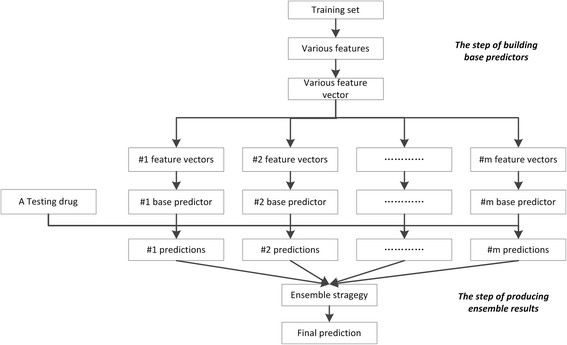
\includegraphics[width=.4\textwidth]{Gambar/gambar4.png}
\caption{Flowchart Algoritma ensemble learning}
\end{figure}

\subsection{ Intrusion Detection System (IDS)}\label{IDS}

Intrusion Detection System adalah sebuah metode yang dapat digunakan untuk mendeteksi aktivitas yang mencurigakan dalam sebuah sistem atau jaringan. IDS dapat melakukan inspeksi terhadap lalu lintas inbound dan outbound dalam sebuah sistem atau jaringan, melakukan analisis dan mencari bukti dari percobaan intrusi dan IDS merupakan sistem untuk mendeteksi adanya “intrusion”
yang dilakukan oleh “intruder” atau “pengganggu atau
penyusup” di jaringan. IDS (Intrusion Detection System)
sangat mirip seperti alarm, yaitu IDS (Instrusion Detection System) akan memperingati bila terjadinya atau adanya
penyusupan pada jaringan. IDS (Intrusion Detection System)
dapat didefinisikan sebagai kegiatan yang bersifat anomaly,
incorrect, inappropriate yang terjadi di jaringan atau host. IDS
(Intrusion Detection System) adalah sistem keamanan yang
bekerja bersama Firewall untuk mengatasi Intrusion.


\begin{figure}
\centering
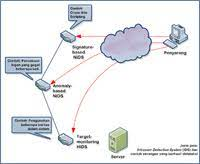
\includegraphics[width=.4\textwidth]{Gambar/gambar6.jpg}
\caption{Jaringan IDS}
\end{figure}

\section{Metodologi}

Metodologi adalah ilmu-ilmu/cara yang digunakan untuk memperoleh kebenaran menggunakan penelusuran dengan tata cara tertentu dalam menemukan kebenaran, tergantung dari realitas yang sedang dikaji. Metodologi tersusun dari cara-cara yang terstruktur untuk memperoleh ilmu.

\begin{figure}
\centering
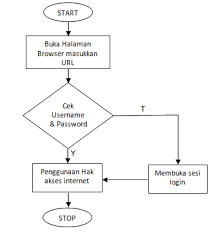
\includegraphics[width=.4\textwidth]{Gambar/gambar5.png}
\caption{contoh tahapan}
\end{figure}

\subsection{Random Forest}
Random Forest merupakan salah satu metode yang digunakan untuk menyelesaikan permasalahan. Metode ini merupakan metode pohon gabungan yang berasal dari metode
classification and regression tree (CART) dan didasarkan pada
teknik pohon keputusan (decision tree), sehingga mampu mengatasi masalah non-linier. Dalam random forest, banyak pohon
ditumbuhkan, sehingga terbentuk suatu hutan (forest). Analisis
selanjutnya akan dilakukan pada kelompok hutan tersebut.

\subsection{K-Nearest Neighbor}
Algoritma K-Nearest Neighbor (K-NN) adalah sebuah
metode klasifikasi terhadap sekumpulan data berdasarkan
pembelajaran data yang sudah terklasifikasikan sebelumya.
Termasuk dalam supervised learning, dimana hasil query
instance yang baru diklasifikasikan berdasarkan mayoritas
kedekatan jarak dari kategori yang ada dalam K-NN.
Tahapan Langkah Algoritma K-NN

• Menentukan parameter k (jumlah tetangga paling dekat).

• Menghitung kuadrat jarak eucliden objek terhadap data
training yang diberikan.

• Mengurutkan hasil no 2 secara ascending (berurutan dari
nilai tinggi ke rendah)

• Mengumpulkan kategori Y (Klasifikasi nearest neighbor
berdasarkan nilai k)

• Dengan menggunakan kategori nearest neighbor yang
paling mayoritas maka dapat dipredisikan kategori objek.

\subsection{Structural Risk Minimization (SVM)}
SVM digunakan untuk mencari hyperplane terbaik dengan
memaksimalkan jarak antar kelas. Hyperplane adalah sebuah
fungsi yang dapat digunakan untuk pemisah antar kelas.
Dalam 2-D fungsi yang digunakan untuk klasifikasi antar
kelas disebut sebagai line whereas, fungsi yang digunakan
untuk klasifikasi antas kelas dalam 3-D disebut plane similarly,
sedangan fungsi yang digunakan untuk klasifikasi di dalam
ruang kelas dimensi yang lebih tinggi di sebut hyperplane.

\begin{figure}
\centering
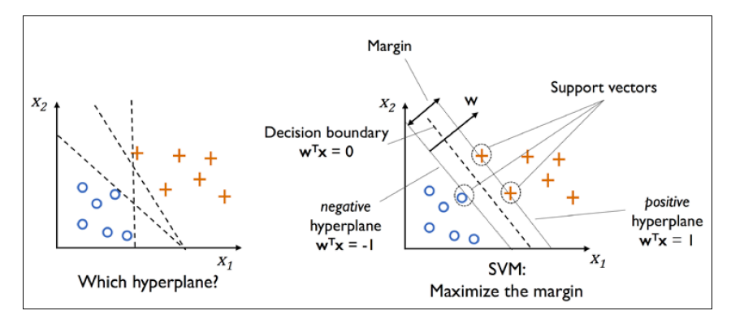
\includegraphics[width=.4\textwidth]{Gambar/gambar8.png}
\caption{contoh hyperplane}
\end{figure}

\section{Hasil dan Pembahasan}

Dalam penelitian ini, ka

\section{Kesimpulan}

Dalam penelitian ini, kami membandingkan beberapa model
untuk sistem deteksi trusi menggunakan Random Forest, KNeighbors, Support Vector Machine, dan Ensemble Learning
dengan ketiga model diatas. Performa keempat pendekatan ini
telah diamati berdasarkan accuracy, precision, recall, dan fmeasure (F1-score).
Dari hasil pengujian dari masing-masing algoritma yang
ada pada tabel, menunjukkan kemampuan klasifikasi algoritma
Ensemble Learning lebih tinggi tingkat akurasi dan ketepatan.
Hasil penelitian ini sangat berguna untuk penelitian masa
depan dengan cara memaksimalkan tingkat kinerja serta meminimalkan tingkat false negative.

Pada saat keamanan komputer sangat penting. salah satu
cara meningkatkan keamanan komputer adalah kita menggunakan IDS. Ada beberapa algoritma yang dapat digunakan,
masing-masing algoritama memiliki kelebihan dan kekurangan. Dengan tersebut keamanan komputer akan terus terjaga.

\bibliographystyle{IEEEtran}
\bibliography{referensi.bib}

<<<<<<< HEAD
\section{REFERENSI}

[1] https://www.dicoding.com/blog/client-server-adalah/

[2] https://mti.binus.ac.id/2019/02/15/keamanan-komputer/

[3] https://informatikalogi.com/algoritma-k-nn-k-nearest-neighbor/
https://medium.com/@samsudiney/penjelasan-sederhana-tentang-apa-itu-svm-149fec72bd02

[4] E. Xydas, C. Marmaras, L. Cipcigan, A. Sani Hassan, and N. Jenkins,
“Forecasting electric vehicle charging demand using support vector machines,” Proceedings of the Universities Power Engineering Conference,pp. 1–6, 09 2013.

[5] W. Zhang, F. Liu, L. Longqiang, and J. Zhang, “Predicting drug side
effects by multi-label learning and ensemble learning,” BMC Bioinformatics, vol. 16, 11 2015.

[6] Mamcose, “Nsl-kdd-network-intrusion-detection,” 2019.

[7] N. Nurhadi, Aplikasi Intelligence Intrusion Detection System (IIDS)
Dengan Menggunakan Metode K-Nearest Neighbor Untuk Mendeteksi
Serangan Pada Jaringan. PhD thesis, Universitas Islam Negeri Sultan
Syarif Kasim Riau, 2017

[8] https://medium.com/@samsudiney/penjelasan-sederhana-tentang-apa-itu-svm-149fec72bd02
=======
>>>>>>> b940c59d55380d6a1f0b328c0df79cc55cce8479

\end{document}
